\expandafter\ifx\csname ifdraft\endcsname\relax
    %!TEX encoding = UTF-8
% +++
% latex = "uplatex"
% +++
\documentclass[uplatex,dvipdfmx,b5j,openany]{jsbook}
\usepackage{graphicx}

\usepackage{siunitx}		%for use si unit
\usepackage{here}			%for use figure here
\usepackage{tikz}			%for use TikZ package
\usepackage{pgfplots}		%for use PGFplots
\usepackage{dcolumn}		%for use significant figures in the table
\usepackage{csvsimple}		%for import csv files
\usepackage[RPvoltages,americanresistors,americaninductors,europeanvoltage,americancurrents]{circuitikz}
\usepackage[noto]{pxchfon}	%for use Noto fonts

% To out put TikZ logo
\usepackage{bxtexlogo}
\bxtexlogoimport{TikZ}

\usepackage{wrapfig}
\usepackage[top=1.5cm, bottom=1.5cm, left=2.5cm, right=2cm]{geometry}

% framed settings
\usepackage{framed}
\definecolor{shadecolor}{gray}{0.80}

% mdframed settings
\usepackage[xcolor,framemethod=tikz]{mdframed}
\usetikzlibrary{shadows}
\mdfdefinestyle{bash}{linecolor=black,linewidth=0.5pt}
\mdfdefinestyle{shadow}{linewidth=0pt,backgroundcolor=black!15}

\usepackage[customcolors]{hf-tikz}
\hfsetfillcolor{black!5}
\hfsetbordercolor{black!50}

\usepackage[cache=false]{minted}

\usepackage{uri}

\tikzset{% tikz style set
  	pointtype triangle/.style={mark=triangle*,mark size=4pt},
  	every mark/.style={fill=white,solid},
  	south west label/.style={
		matrix,matrix of nodes,
		anchor=south west,at={(rel axis cs:0.01,0.01)},
		nodes={anchor=west,inner sep=0},
  	},
}

\pgfplotsset{% graph style set
    table/col sep=comma, % Use CSV files
  	compat=1.12,
  	major tick length=0.2cm,
  	minor tick length=0.1cm,
  	every axis/.style={semithick},
  	tick style={semithick,black},
  	legend cell align=left,
  	legend image code/.code={%
		\draw[mark repeat=2,mark phase=2,#1]
	  	plot coordinates {(0cm,0cm) (0.5cm,0cm) (1.0cm,0cm)};
  	},
  	log number format basis/.code 2 args={
	\pgfmathsetmacro\e{#2}
	\pgfmathparse{#2==0}\ifnum\pgfmathresult>0{1}\else
	\pgfmathparse{#2==1}\ifnum\pgfmathresult>0{10}\else
	{$#1^{\pgfmathprintnumber{\e}}$}\fi\fi},
}

% macros
\newcommand{\logoLaTeX}{{\rm \textbf \LaTeX}\hspace{0zw}}
	\graphicspath{{./figure/}}
	\begin{document}
\fi

\chapter{はじめに}
	お手に取って頂きありがとうございます。

	みなさんは\LaTeX \footnote{ラテック/ラテフ、英語圏ではレイテックとも読まれる}というソフトウェアをご存知でしょうか?
	\LaTeX とは\TeX \footnote{テック/テフと読む}を元に開発された文書作成ソフトウェアで、
	編集している画面が出力として得られるMicrosoft Wordなどのソフトウェアとは対照的に
	\LaTeX の文書はプログラミング言語のような形で命令と文章を記述し、
	タイプセットと呼ばれるコンパイルを行うことでPDF形式での出力を得られる、という形の文書作成システムです。

	\LaTeX には多くの拡張機能があり、化学記号を美しく出力するための機能、
	音楽記号を美しく出力するための機能など様々な機能が存在します。
	本書では、回路図を美しく出力するための拡張機能であるCircui{\TikZ}\footnote{サーキッティクスと読む}を取り扱います。

	\begin{figure}[H]
		\centering
		\begin{tabular}{c}
			\begin{minipage}{0.45\hsize}
				\centering
				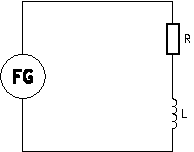
\includegraphics[width=4cm]{circuit.pdf}
				\caption{KiCadで生成した回路図}
				\label{fig:kicad-circuit}
			\end{minipage}

			\begin{minipage}{0.45\hsize}
				\centering
				\begin{circuitikz}[scale=1.5]
					\draw (0,0)
					to[sV,l=$FG$] (0,2);
					\draw (0,2)
					to[short] (2,2);
					\draw (2,2)
					to[R,l_=$R$] (2,1);
					\draw (2,1)
					to[L,l_=$L$] (2,0);
					\draw (2,0)
					to[short] (0,0);
				\end{circuitikz}
				\caption{Circui{\TikZ}で生成した回路図}
				\label{fig:circuitikz-circuit}
			\end{minipage}
		\end{tabular}
	\end{figure}

	図\ref{fig:kicad-circuit}は、一般的な回路図エディタであるKiCadを用いて作成した回路図、
	図\ref{fig:circuitikz-circuit}は、Circui{\TikZ}で作成した回路図です。
	Circui{\TikZ}を用いれば、このように教科書などの書籍でみられるような美しい回路図をあなたの手で作成することができます。

	本書がきっかけで\LaTeX に興味を持っていただければと思います。

\expandafter\ifx\csname ifdraft\endcsname\relax
	\end{document}
\fi